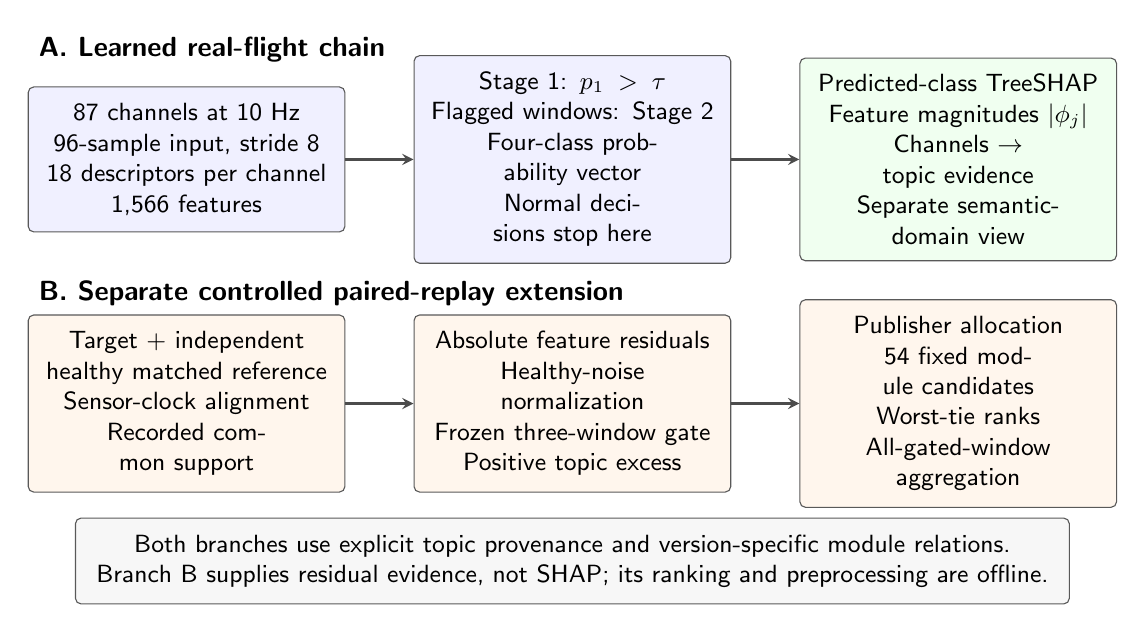
\begin{tikzpicture}[
 font=\sffamily\small,
 box/.style={draw=black!65,rounded corners=2pt,align=center,text width=3.6cm,minimum height=1.65cm,inner sep=6pt},
 arrow/.style={->,>=stealth,line width=0.8pt,draw=black!70}]
\node[anchor=west,font=\sffamily\bfseries] at (-0.1,5.5) {A. Learned real-flight chain};
\node[box,fill=blue!6] (a) at (1.9,4.1) {87 channels at 10 Hz\\96-sample input, stride 8\\18 descriptors per channel\\1,566 features};
\node[box,fill=blue!6] (b) at (6.8,4.1) {Stage 1: $p_1>\tau$\\Flagged windows: Stage 2\\Four-class probability vector\\Normal decisions stop here};
\node[box,fill=green!6] (c) at (11.7,4.1) {Predicted-class TreeSHAP\\Feature magnitudes $|\phi_j|$\\Channels $\rightarrow$ topic evidence\\Separate semantic-domain view};
\draw[arrow] (a)--(b);\draw[arrow] (b)--(c);
\node[anchor=west,font=\sffamily\bfseries] at (-0.1,2.4) {B. Separate controlled paired-replay extension};
\node[box,fill=orange!7] (d) at (1.9,1.0) {Target + independent\\healthy matched reference\\Sensor-clock alignment\\Recorded common support};
\node[box,fill=orange!7] (e) at (6.8,1.0) {Absolute feature residuals\\Healthy-noise normalization\\Frozen three-window gate\\Positive topic excess};
\node[box,fill=orange!7] (f) at (11.7,1.0) {Publisher allocation\\54 fixed module candidates\\Worst-tie ranks\\All-gated-window aggregation};
\draw[arrow] (d)--(e);\draw[arrow] (e)--(f);
\node[box,text width=12.2cm,minimum height=0.85cm,fill=black!3] at (6.8,-1.0) {Both branches use explicit topic provenance and version-specific module relations.\\Branch B supplies residual evidence, not SHAP; its ranking and preprocessing are offline.};
\end{tikzpicture}
